\chapter{Solução Proposta}\label{cap:solucao}

Uma vez que o conhecimento teórico necessário para o entendimento completo do trabalho já foi apresentado, neste capítulo será definida a solução proposta.

A solução desenvolvida consiste em um algoritmo analisa imagens de vídeo de um estacionamento descoberto e determina o número de vagas livres na imagem, além da sua localização aproximada. O sistema funciona bem em imagens de menor qualidade, mas é necessário que o vídeo adquirido seja em cores.

O trabalho se preocupa em cumprir os critérios definidos no capítulo \ref{cap:trabalhos}. Além disso, o sistema foi desenvolvido de forma que pudesse processar as imagens adquiridas de forma mais próxima possível do tempo real, causando o mínimo de atrasos para o processamento de quadros subsequentes do vídeo.

O sistema recebe como entrada um vídeo em cores capturado em um certo ângulo e um vetor de regiões de interesse no vídeo. A saída do programa a cada quadro é o número de vagas livres em cada região de interesse no vídeo.

A imagem \ref{fig:fluxograma} contém um fluxograma que mostra as etapas do processamento de cada quadro do vídeo adquirido. No decorrer deste capítulo cada um desses passo será discutido com mais detalhes.

\begin{figure}
	\centering
	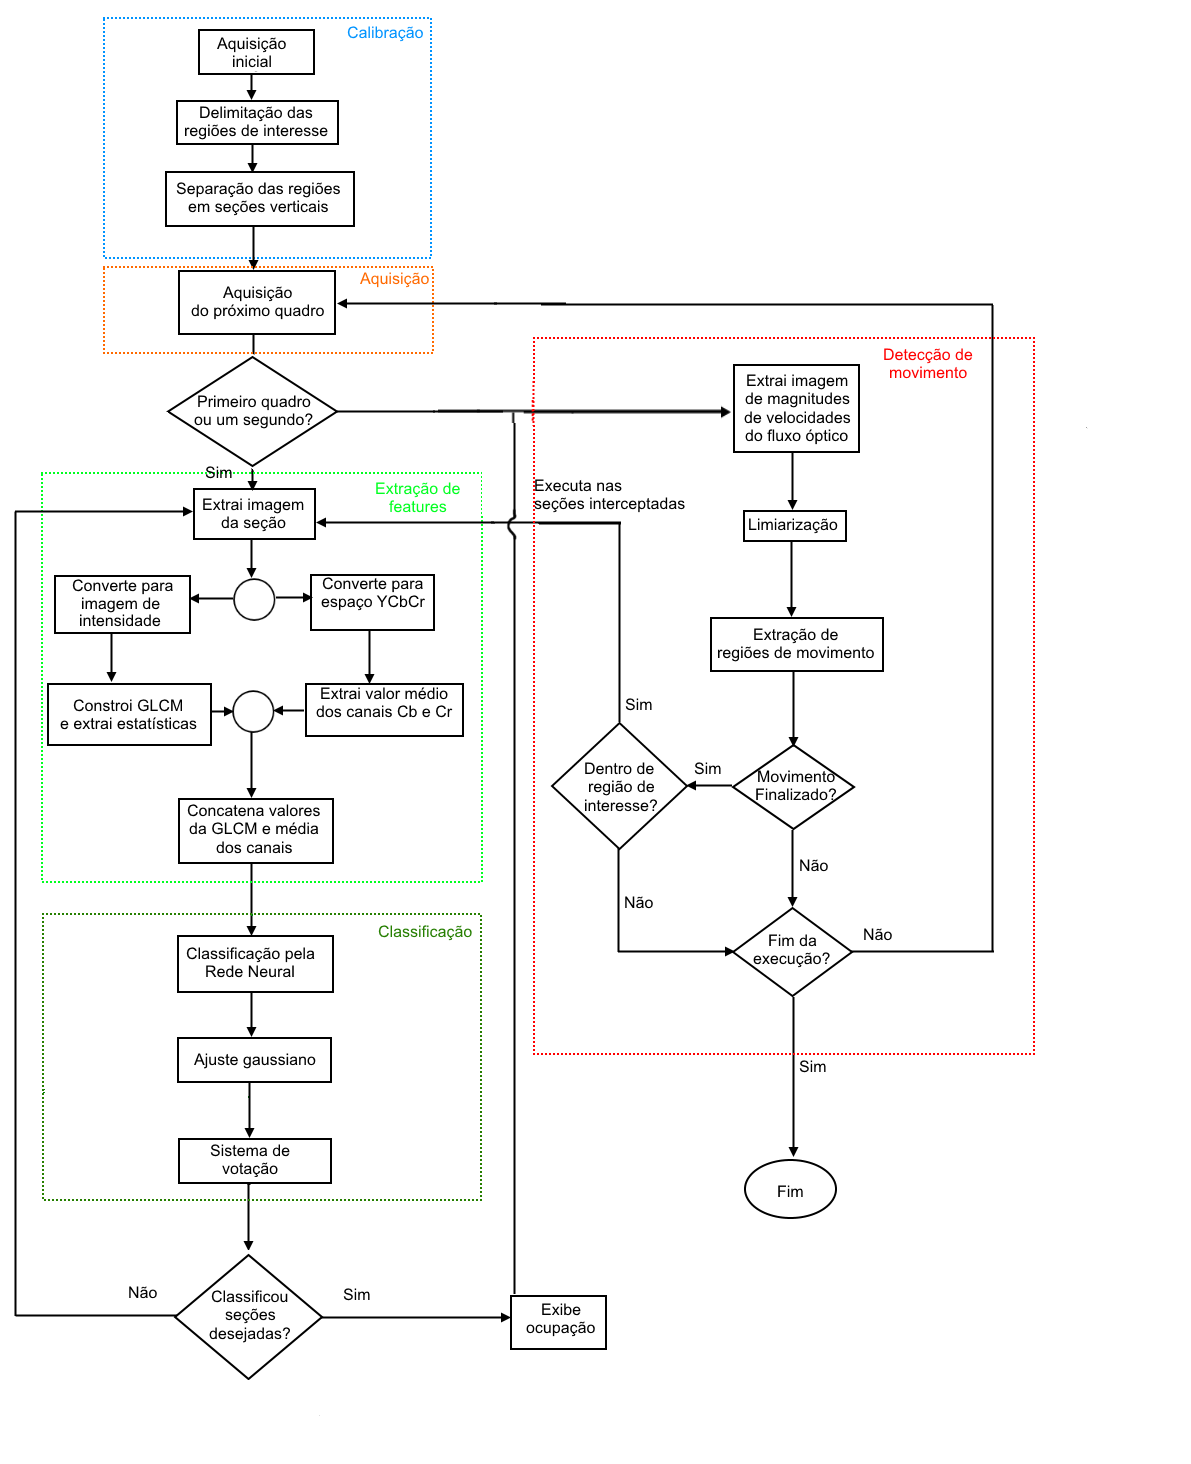
\includegraphics[width=1\textwidth]{fluxograma}
	\label{fig:fluxograma}
	\caption{Um fluxograma com o funcionamento geral do programa}
	\centering
\end{figure}



\section{Aquisição}\label{sec:aquisicao}

Uma câmera montada em um poste de luz ou outro ponto similar captura as imagens utilizadas pelo programa. A câmera é montada de forma que o seu campo de visão contenha o máximo de vagas possível, porém que ainda seja possível visualizar o asfalto das vagas desocupadas e ocorra o mínimo de oclusão de veículos. A figura \ref{fig:aquisicao} mostra um quadro de uma aquisição em ângulo ideal.

\begin{figure}[!ht]
	\centering
	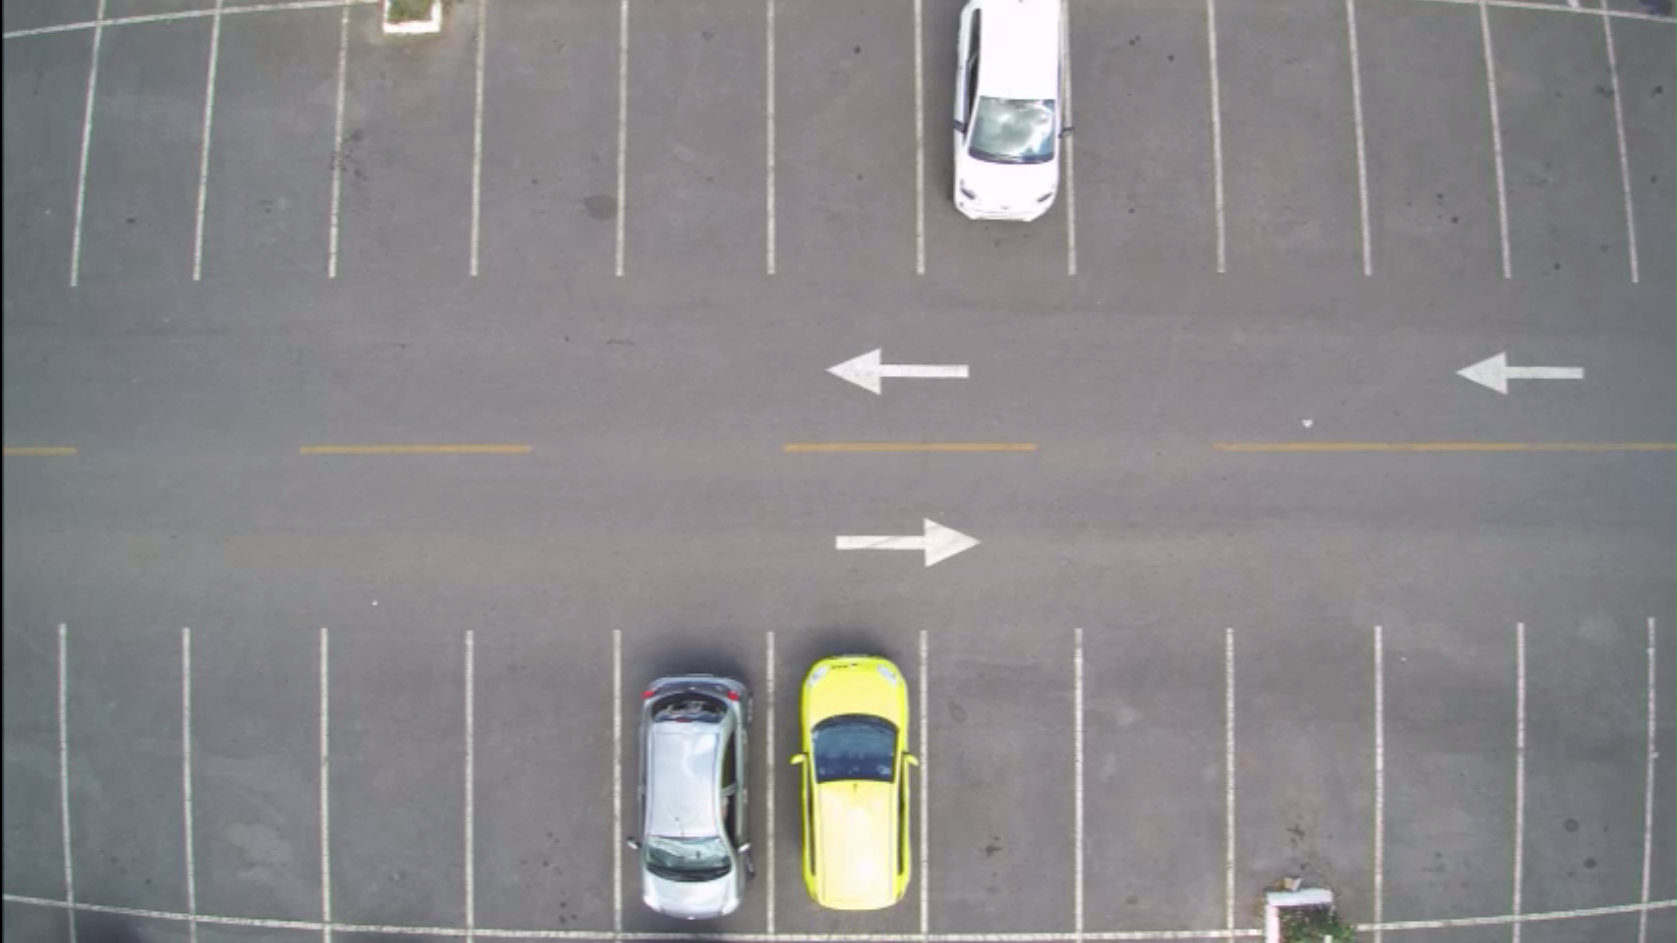
\includegraphics[width=8cm]{Vazio3}
	\label{fig:aquisicao}
	\caption{Um quadro de um vídeo adquirido por uma câmera do sistema}
	\centering
\end{figure}

Neste trabalho, a preocupação foi implementar um programa que analisa as imagens de uma única câmera de vídeo. Em uma aplicação no mundo real, diversas câmeras seriam instaladas para aumentar a cobertura do estacionamento. Neste caso, cada vídeo seria processado por uma cópia diferente do sistema, responsável pela área coberta pela câmera correspondente. As saídas de cada cópia do programa correspondem a ocupação das vagas em um setor diferente do estacionamento.

\section{Regiões de Interesse}\label{sec:ROIs}

No momento da instalação do programa, é necessário definir um número qualquer de regiões de interesse(\textit{Regions of interest} ou ROIs). Essas regiões determinam a área da imagem onde existem vagas. Além de determinar as regiões, deve-se informar ao programa o número de vagas existente em cada região de interesse.

As ROIs devem ser retangulares e determinadas de forma a não haver interseção entre elas, como exemplificado na figura \ref{fig:ROIs} que mostra as regiões determinadas para o quadro da figura \ref{fig:aquisicao}.

\begin{figure}
	\centering
	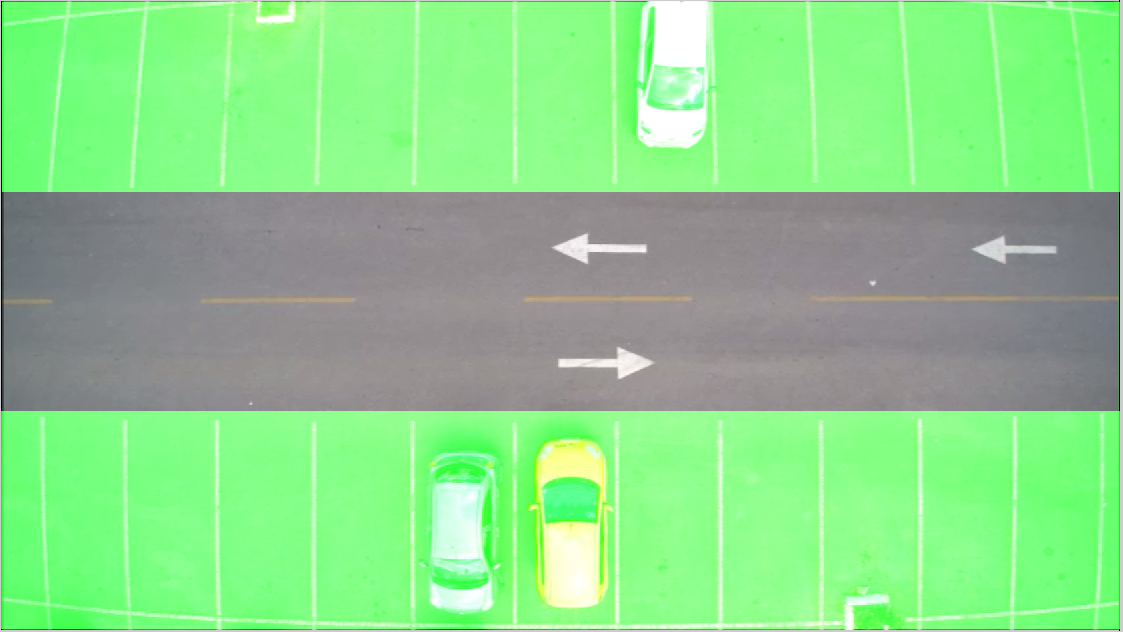
\includegraphics[width=8cm]{ROIs}
	\label{fig:ROIs}
	\caption{O mesmo quadro da figura \ref{fig:aquisicao}, depois de definidas as regiões de interesse, marcadas de verde.}
	\centering
\end{figure}

Depois de determinadas as regiões de interesse, cada uma delas é dividida em um número igual de seções verticais como ilustrado na figura \ref{fig:secoesVerticais}. Como as vagas não são determinadas individualmente no momento da instalação do programa, é necessário que seja feita alguma divisão das ROIs. Cada uma destas seções verticais é classificada separadamente em uma etapa futura do processamento. O resultado da classificação de cada seção de uma ROI determina um vetor $v$ de $n$ elementos, onde $n$ é o número de seções em que a região foi dividida e cada elemento indica a ocupação da vaga, sendo o valor $1$ correspondente a uma vaga ocupada e o valor $2$ correspondente a uma vaga livre. Através da análise deste vetor é que o programa determina o número de vagas livres em cada região. Munido do número de vagas que cada região contém e um valor aproximado do número de seções que um carro ocupa, o programa estima quantas vagas estão ocupadas, e encontra o número de vagas livres através de simples subtração e a posição aproximada destas vagas através da posição das seções livres no vetor.

\begin{figure}
	\centering
	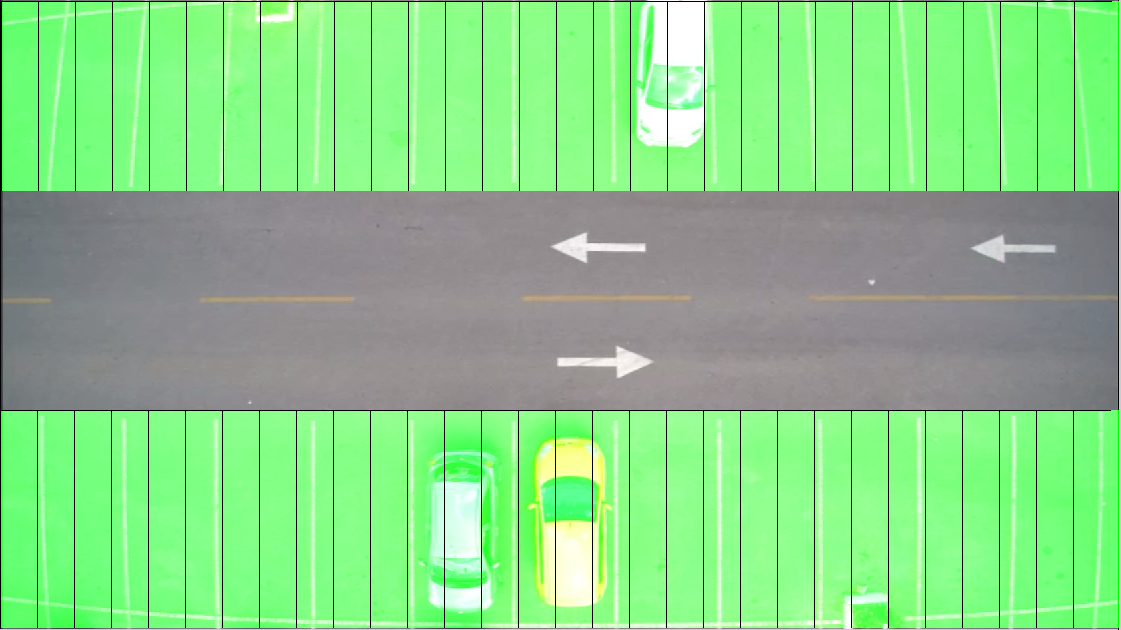
\includegraphics[width=8cm]{Secoes}
	\label{fig:secoesVerticais}
	\caption{As ROIs determinadas na figura \ref{fig:ROIs} separadas em trinta seções verticais que ainda não foram classificadas. Nesta etapa os vetores $v$ de cada região é composto de trinta valores $2$.}
	\centering
\end{figure}


\section{Classificação das seções} \label{sec:classificacao}


\subsection{Extração de características}


\subsection{Classificação da rede neural artificial}

\subsection{Ajuste gaussiano dos vizinhos}

\subsection{Sistema de votação}


\section{Extração do movimento}

\subsection{Fluxo Óptico}

\subsection{Regiões de movimento}





